\documentclass[9pt,twocolumn,twoside,lineno]{pnas-new}
% Use the lineno option to display guide line numbers if required.
% Note that the use of elements such as single-column equations
% may affect the guide line number alignment. 

%%Nadir's Shortcuts
\newcommand{\beqn}{\begin{equation}}
\newcommand{\eeqn}{\end{equation}}
\newcommand{\beqa}{\begin{eqnarray}}
\newcommand{\eeqa}{\end{eqnarray}}
\newcommand{\beqanonum}{\begin{eqnarray*}}
\newcommand{\eeqanonum}{\end{eqnarray*}}
\newcommand{\beqnonum}{\begin{equation*}}
\newcommand{\eeqnonum}{\end{equation*}}
\newcommand{\jump}{\vspace{0.5cm}}
\newcommand{\bbf}{\begin{bf}}
\newcommand{\ebf}{\end{bf}}
\newcommand{\eqnref}[1]{(\ref{#1})}
\newcommand{\defn}[1]{\begin{bf}\emph{#1}\end{bf}}
\newcommand{\reals}{\ensuremath{\mathbb{R}}}
\newcommand{\complex}{\ensuremath{\mathbb{C}}}
\newcommand{\integers}{\ensuremath{\mathbb{Z}}}
\newcommand{\half}{\ensuremath{\frac{1}{2}}}
\newcommand{\n}{\nonumber}
\newcommand{\inverse}{^{-1}}
\newcommand{\comment}[1]{\textcolor{blue}{[{#1}]}}

%calculus shorthand
\newcommand{\timeder}{\frac{d}{dt}}
\newcommand{\partialder}[1]{\frac{\partial}{\partial #1}}
\newcommand{\partialderf}[2]{\ensuremath{\frac{\partial #1}{\partial #2}}}
\newcommand{\der}[2]{\ensuremath{\frac{d #1}{d #2}}}
\newcommand{\dx}{\ensuremath{\frac{d}{dx}}}
\newcommand{\ddx}{\ensuremath{\frac{d}{dx}}}
\newcommand{\kvec}{\ensuremath{\vec{k}}}
\newcommand{\uvec}{\ensuremath{\mathbf{u}}}
\newcommand{\zhat}{\ensuremath{\mathbf{\hat{z}}}}
\newcommand{\khat}{\ensuremath{\mathbf{\hat{k}}}}
\newcommand{\unitvect}[1]{\ensuremath{\mathbf{\hat{#1}}}}
\newcommand{\ppx}{\ensuremath{\partial_x}}
\newcommand{\ppy}{\ensuremath{\partial_y}}
\newcommand{\ppz}{\ensuremath{\partial_z}}
\newcommand{\ppt}{\ensuremath{\partial_T}}
\newcommand{\ppp}{\ensuremath{\partial_p}}


% radiation shorthand
\newcommand{\cotwo}{\ensuremath{\mathrm{CO_2}}}
\newcommand{\othree}{\ensuremath{\mathrm{O_3}}}
\newcommand{\htwo}{\ensuremath{\mathrm{H_2O}}}
\newcommand{\QLW}{\ensuremath{Q_\mathrm{LW}}}
\newcommand{\QSW}{\ensuremath{Q_\mathrm{SW}}}
\newcommand{\Qnet}{\ensuremath{Q_\mathrm{net}}}
\newcommand{\FLW}{\ensuremath{F^\mathrm{LW}}}
\newcommand{\FSW}{\ensuremath{F^\mathrm{SW}}}
\newcommand{\FLWgl}{\ensuremath{F^\mathrm{LW}_{\mathrm{gl}}}}
\newcommand{\FSWgl}{\ensuremath{F^\mathrm{SW}_{\mathrm{gl}}}}
\newcommand{\USW}{\ensuremath{U^\mathrm{SW}}}
\newcommand{\DSW}{\ensuremath{D^\mathrm{SW}}}
\newcommand{\Fnet}{\ensuremath{F^\mathrm{net}}}
\newcommand{\Fnetgl}{\ensuremath{F^\mathrm{net}_{\mathrm{gl}}}}
\newcommand{\Fgl}{\ensuremath{F_{\mathrm{gl}}}}
\newcommand{\olr}{\ensuremath{\mathrm{OLR}}}
\newcommand{\OLR}{\ensuremath{\mathrm{OLR}}}
\newcommand{\trans}{\ensuremath{\mathcal{T}}}
\newcommand{\solar}{\ensuremath{I_0}}
\newcommand{\cool}{\ensuremath{\mathcal{C}}}
\newcommand{\cminverse}{\ensuremath{\mathrm{cm^{-1}}}}
\newcommand{\pierre}{P10}
\newcommand{\tauk}{\ensuremath{\tau_\lambda}}

% Units
\newcommand{\Wmsq}{\ensuremath{\mathrm{W/m^2}}}
\newcommand{\WmsqK}{\ensuremath{\mathrm{W/m^2/K}}}
\newcommand{\meter}{\ensuremath{\mathrm{m}}}
\newcommand{\kg}{\ensuremath{\mathrm{kg}}}
\newcommand{\Kinverse}{\ensuremath{\mathrm{K^{-1}}}}
\newcommand{\Kelvin}{\ensuremath{\mathrm{K}}}

% meteorology shorthand
\newcommand{\qv}{\ensuremath{q}}
\newcommand{\rhov}{\ensuremath{\rho_\mathrm{v}}}
\newcommand{\Hv}{\ensuremath{H_\mathrm{v}}}
\newcommand{\Rv}{\ensuremath{R_\mathrm{v}}}
\newcommand{\qa}{\ensuremath{q_a}}
\newcommand{\qvstar}{\ensuremath{q^*}}
\newcommand{\pvstar}{\ensuremath{p^*_{\mathrm{v}}}}
\newcommand{\Ta}{\ensuremath{T_a}}
\newcommand{\Tav}{\ensuremath{T_\mathrm{av}}}
\newcommand{\Ts}{\ensuremath{T_\mathrm{s}}}
\newcommand{\Tsgl}{\ensuremath{T_\mathrm{s,gl}}}
\newcommand{\ps}{\ensuremath{p_s}}
\newcommand{\RH}{\ensuremath{\mathrm{RH}}}
\newcommand{\cld}{\ensuremath{\mathrm{Cld}}}
\newcommand{\WVP}{\ensuremath{\mathrm{WVP}}}
\newcommand{\ztop}{\ensuremath{z_\mathrm{top}}}
\newcommand{\ztp}{\ensuremath{z_\mathrm{tp}}}
\newcommand{\zlcl}{\ensuremath{z_\mathrm{LCL}}}
\newcommand{\Tlcl}{\ensuremath{T_\mathrm{LCL}}}
\newcommand{\Ttp}{\ensuremath{T_\mathrm{tp}}}
\newcommand{\Text}{\ensuremath{T_\mathrm{ext}}}
\newcommand{\ptp}{\ensuremath{p_\mathrm{tp}}}
\newcommand{\lapseav}{\ensuremath{\Gamma_\mathrm{av}}}
\newcommand{\gammaav}{\ensuremath{\Gamma_\mathrm{av}}}
\newcommand{\Htauk}{\ensuremath{H_{\tau_k}}}
\newcommand{\east}{\ensuremath{\mathrm{E}}}
\newcommand{\north}{\ensuremath{\mathrm{N}}}
\newcommand{\south}{\ensuremath{\mathrm{S}}}
\newcommand{\tav}{\ensuremath{t_\mathrm{av}}}
\newcommand{\kmax}{\ensuremath{k_\mathrm{max}}}
\newcommand{\kmin}{\ensuremath{k_\mathrm{min}}}

%Variables
%\newcommand{\figurepath}{../../../figures/}
\newcommand{\figurepath}{./}



\templatetype{pnasresearcharticle} % Choose template 
% {pnasresearcharticle} = Template for a two-column research article
% {pnasmathematics} = Template for a one-column mathematics article
% {pnasinvited} = Template for a PNAS invited submission

\title{Mean Precipitation Change from a Deepening Troposphere}

% Use letters for affiliations, numbers to show equal authorship (if applicable) and to indicate the corresponding author
\author[a,b,c]{Nadir Jeevanjee}
\author[d,e]{David M. Romps} 


\affil[a]{Department of Geosciences, Princeton University, Princeton NJ 08544 USA}
\affil[b]{Princeton Program in Atmosphere and Ocean Sciences, Princeton University, Princeton NJ 08540 USA}
\affil[c]{Geophysical Fluid Dynamics Laboratory,  Princeton NJ  08540 USA}
\affil[d]{Department of Earth and Planetary Science, University of California at Berkeley, Berkeley, CA 94702  USA}
\affil[e]{Climate and Ecosystems Sciences Division, Lawrence Berkeley National Laboratory, Berkeley, CA USA}

% Please give the surname of the lead author for the running footer
\leadauthor{Jeevanjee} 

% Please add here a significance statement to explain the relevance of your work
\significancestatement{Global climate models robustly predict that global mean precipitation should increase at roughly 2-3 \% \Kinverse, but the origin of these values is not well understood. Here we develop a simple theory to help explain these values. This theory suggests that global mean precipitation is closely tied to the depth of the troposphere, when measured in temperature coordinates. When surface temperatures increase, this `temperature depth' of the troposphere also increases, causing an increase in global mean precipitation.}

% Please include corresponding author, author contribution and author declaration information
\authorcontributions{N.J. and D.M.R. designed research and analyzed data. N.J. wrote the paper.}
\authordeclaration{The authors declare no conflict of interest.}
%\equalauthors{\textsuperscript{1}}
\correspondingauthor{\textsuperscript{2}To whom correspondence should be addressed. E-mail: nadirj\@princeton.edu}

% Keywords are not mandatory, but authors are strongly encouraged to provide them. If provided, please include two to five keywords, separated by the pipe symbol, e.g:
\keywords{Climate Change $|$ Atmospheric Science $|$ Hydrological Cycle $|$} 

\begin{abstract}
Global climate models robustly predict that global mean precipitation should increase at roughly 2-3 \% \Kinverse, but the origin of these values is not well understood. Here we develop a simple theory to help explain these values. This theory combines the well-known radiative constraint on precipitation, which says that condensation heating from precipitation is balanced by the net radiative cooling of the free troposphere, with an invariance of radiative cooling profiles when expressed in temperature coordinates. These two constraints yield a picture in which mean precipitation is controlled primarily by the depth of the troposphere, when measured in temperature coordinates. We develop this theory in idealized simulations of radiative-convective equilibrium, and  also demonstrate its applicability to global climate models.  \end{abstract}

\dates{This manuscript was compiled on \today}
\doi{\url{www.pnas.org/cgi/doi/10.1073/pnas.XXXXXXXXXX}}

\begin{document}

% Optional adjustment to line up main text (after abstract) of first page with line numbers, when using both lineno and twocolumn options.
% You should only change this length when you've finalised the article contents.
\verticaladjustment{-2pt}

\maketitle
\thispagestyle{firststyle}
\ifthenelse{\boolean{shortarticle}}{\ifthenelse{\boolean{singlecolumn}}{\abscontentformatted}{\abscontent}}{}
% If your first paragraph (i.e. with the \dropcap) contains a list environment (quote, quotation, theorem, definition, enumerate, itemize...), the line after the list may have some extra indentation. If this is the case, add \parshape=0 to the end of the list environment.
%\dropcap{T}his PNAS journal template is provided to help you write your work in the correct journal format.  Instructions for use are provided below.
%
%Note: please start your introduction without including the word ``Introduction'' as a section heading (except for math articles in the Physical Sciences section); this heading is implied in the first paragraphs. 
Despite its fundamental role in driving atmospheric motions, atmospheric radiative cooling remains somewhat enigmatic. Though the fundamentals of radiative transfer are well-understood, translating these fundamentals into realistic cooling rates requires complicated radiative transfer calculations which render the final result somewhat inscrutable. As a result, we lack simple descriptions of the radiative cooling profiles produced by our numerical models.

One implication is that quantities that are closely tied to radiative cooling, such as global mean precipitation, also remain somewhat enigmatic. We do know that the atmospheric (rather than planetary) energy budget, in which condensation heating from precipitation balances atmospheric radiative cooling, constrains global mean precipitation $P$ to be roughly equal to column-integrated net radiative cooling $\Qnet$ \cite{ogorman2012,allen2002,mitchell1987}:
\beqn
	LP \approx \Qnet \quad \mbox{(\Wmsq)} \label{rad_precip_constraint}
\eeqn
(here $L$ is the latent heat of vaporization and we neglect surface sensible heat fluxes, a point we return to below). We also know that  global climate models robustly exhibit  increases in $P$ with warming of $2 -3\%\ \Kinverse$  \cite{stephens2008a, lambert2008, held2006}. Furthermore, recent work  has attributed this increase to an increase in downward radiative emission from the atmosphere at the surface \cite{stephens2010, pendergrass2014, takahashi2009}. Despite this progress, however, a basic question remains unanswered: why does this increase take on the value that it does? Why $2 -3\%\ \Kinverse$ and not many times  larger or smaller?

This paper aims to reveal some simple behavior in radiative cooling profiles, and to use it to  answer this question about precipitation change. We will  focus on how vertically-resolved radiative cooling profiles change with warming, rather than focusing on radiative fluxes at the surface or top-of-atmosphere. In particular, we will argue, following \cite{simpson1928,ingram2010}, that water vapor density and optical depth profiles should behave simply when considered as functions of temperature as a vertical coordinate. This implies  that LW and SW radiative flux divergences should also behave simply in temperature coordinates. This simple behavior leads to a predictive expression for $d\Qnet/d\Ts$ and hence $dP/d\Ts$ (\Ts\ is surface temperature), which we validate with limited-area cloud-resolving model (CRM) simulations which emulate  the tropical atmosphere. We then seek insight from our results, and also apply them  to global climate models (GCMs). 


This approach leverages the insights of \cite{simpson1928, ingram2010}, but also builds upon their work in various ways. First, we verify some of their ideas using comprehensive radiative transfer calculations, which to our knowledge has not yet been done. We also shift the focus from outgoing longwave radiation (i.e., thermal emission to space) to atmospheric radiative cooling, and also extend their  arguments to include both the longwave (LW, thermal emission) and shortwave (SW, solar radiation) bands. Our work also has precedent in \cite{takahashi2009}, which similarly takes an idealized approach in analyzing the radiative constraint on hydrological sensitivity. That study, however,  used a gray radiation model wherein the concentration of the longwave absorber is not directly tied to temperature, a  link which will prove crucial here (see Eqns. \ref{rhov}-\ref{tauT} below).

\section{CRM Simulations of RCE}
We begin by studying precipitation change in one of the simplest systems in which the radiative constraint on precipitation \eqnref{rad_precip_constraint} operates, namely cloud-resolving radiative-convective equilibrium (RCE). This system is an idealized and isolated version of Earth's tropics, and exhibits precipitation increases of roughly $3 -4\%\ \Kinverse$, similar to the GCM range \cite{romps2011, muller2011b}.  

We simulate RCE using Das Atmosph\"arische Modell \cite[DAM,][]{romps2008}, a fully-compressible, non-hydrostatic cloud-resolving model, coupled to radiation via the comprehensive Rapid Radiative Transfer Model 
\cite[RRTM,][]{mlawer1997}. DAM employs the six-class Lin-Lord-Krueger  microphysics scheme \cite{lin1983, lord1984, krueger1995}, and in contrast to its original formulation in \cite{romps2008} employs no explicit sub-grid scale turbulence scheme, relying instead on `implicit LES'  \citep[][essentially just the existing numerical diffusion]{margolin2006}  for sub-grid scale transport.

	Our RCE simulations ran on a square doubly-periodic domain of horizontal dimension $L=72$ km, with  a horizontal grid spacing of $dx=1$ km. The vertical grid spacing stretched smoothly from 50 m  below 1000 m to 250 m  between 1000 m and 5000 m, and then to 500 m up to the model top at  30 km. We calculated surface heat and moisture fluxes using simple bulk aerodynamic formulae, and used a pre-industrial \cotwo\  concentration of 280 ppm with no ozone. To explore precipitation changes  with warming we ran five experiments at prescribed surface temperatures of $\Ts=(280,290,300,310,320)$ K, though most of our figures omit the 320 K run for clarity. Our runs branched off the equilibrated runs described in \cite{romps2014}, and were run for 60 days  to iron out any artifacts from changing the domain and resolution. All vertical profiles are time-mean and domain-mean, averaged over the last 20 days of each run. These simulations do not exhibit any organization or `self-aggregation' \citep{wing2017} (SI Appendix, Fig. S1).
	
Since we run with prescribed \Ts\ and fixed \cotwo, we are isolating the hydrological sensitivity to \Ts\ and neglecting the rapid adjustment from \cotwo. The former is relatively robust across models and forcing types, whereas rapid adjustments  depend on  forcing type \cite{flaschner2016,samset2017}. The latter contributes roughly -0.5 \Wmsq/K in $4\times \cotwo$ experiments \cite{flaschner2016}, a non-dominant effect. 

%=================================%
% Temperature invariance of flux divergence %
%=================================%
\section{\Ts-invariance of Flux Divergences}
\label{Ts_invariance}
The simple behavior of radiative cooling alluded to above begins with the key fact that  the water vapor density 
	\beqn
		\rhov =  \RH\frac{\pvstar(T)}{\Rv T} \; 
	\label{rhov}
	\eeqn
	 is (up to variations in relative humidity \RH) a function of temperature only. [Note that it has been shown recently that RH is itself a function of $T$ in RCE \cite{romps2014}. Also, here \pvstar\  is the saturation vapor pressure of water, and all other symbols have their usual meaning.] If we use $T$ as a vertical coordinate, \eqref{rhov} then tells us that the function $\rhov(T)$ does not depend on \Ts. This is what we mean by `\Ts-invariance'. We verify the \Ts-invariance of $\rhov(T)$  in our simulations in  Fig. \ref{rhov_fig}, where indeed  the \rhov\ profiles at different \Ts\ collapse onto a single curve when plotted in temperature coordinates.

%Figure rhov_fig
\begin{figure}[t]
	\begin{center}
			\includegraphics[scale=0.4]{\figurepath rhov.pdf}
		\caption{Profiles of $\rhov(T)$ from our RCE simulations at various \Ts, with both linear and log scales. These profiles are `\Ts-invariant' in the sense that $\rhov(T)$ does not depend on \Ts, i.e. that the \rhov\ profiles at different \Ts\ collapse onto a single curve.
		\label{rhov_fig}
		}
	\end{center}
\end{figure}

	For wavelengths  $\lambda$ where water vapor dominates, the optical depth $\tauk$ is just
	\beqn
		\tauk(z) = \kappa(\lambda) \int_z^\infty   \rhov(z') \, dz'  \; 
		\label{tauz}
	\eeqn
		where $\kappa(\lambda)$ is a  mass absorption coefficient  (units $\mathrm{m^2/kg}$) whose pressure-broadening and temperature scaling we neglect \citep[as in ref.][see  also SI text 2]{ingram2010}. Optical depth can be interpreted as minus the logarithm of the transmission function $e^{-\tauk(z)}$, which gives the fraction of radiation emitted at a given height that travels unabsorbed out to space. Changing the integration variable in \eqref{tauz} to temperature $T'$  yields
		\beqn
		\tauk(T) \approx  \kappa(\lambda) \int_{\Ttp}^T   \rhov(T') \, \frac{dT'}{\Gamma}  \; ,
		\label{tauT}
	\eeqn
	where we neglect stratospheric water vapor and take the lower limit of the integral to be the tropopause temperature $\Ttp \approx 185$ K, where radiative cooling goes to 0 (see Fig. \ref{pptfnet_tinv_dam}, which also shows that \Ttp\ is \Ts-invariant). The only quantity in \eqref{tauT} that might still exhibit some \Ts-dependence is the lapse rate $\Gamma\equiv -\frac{dT}{dz}$, but Fig. 2 of \cite{ingram2010} shows that  for moist adiabats typical of the tropics, $\Gamma(T)$ is also fairly  \Ts-invariant. (For GCMs the presence of $\Gamma(T)$ in \eqnref{tauT} will be more significant; see section \ref{sec_GCMs}.) Equation \eqnref{tauT} then implies that \tauk\ profiles at any $\lambda$ exhibit the same \Ts-invariance as \rhov. This argument was also made by \cite{ingram2010}, and its essence goes back to  \cite{simpson1928}. We check its validity with a line-by-line radiative transfer calculation in SI Appendix, Fig. S5.
	
	To build on this and connect it with radiative cooling, we invoke the cooling-to-space  approximation \cite[][]{thomas2002, rodgers1966}, which says that the spectrally resolved LW flux divergence in temperature coordinates $-\ppt \FLW_\lambda$ (units $\Wmsq/\mathrm{K}/\meter$, fluxes positive upward, minus sign introduced for consistent sign with  $\ppz \FLW_\lambda$) is approximately
	\beqn
		-\ppt \FLW_\lambda \approx  \pi B_\lambda(T) e^{-\tauk(T)} \der{\tauk}{T} \ .
	\label{cts_spectral}
	\eeqn
 (Note that RRTM does not employ \eqref{cts_spectral}; we simply use it here as a heuristic.) Since the Planck function $B_\lambda(T)$ is \Ts-invariant, as is the optical depth, we also expect $-\ppt \FLW_\lambda$ to be \Ts-invariant. 

%Figure pptfnet_tinv_dam
\begin{figure}[t]
	\begin{center}
			\includegraphics[scale=0.3]{\figurepath pptfnet_tinv_dam.pdf}
		\caption{Net flux divergence  $-\ppt \Fnet$, as diagnosed from RRTM coupled to our CRM RCE simulations at \Ts=(280,\ 290,\ 300,\ 310) K. Fluxes are plotted from the lifting condensation level of each simulation to 22.5 km for clarity, and  in height, pressure, and temperature coordinates to emphasize the \Ts-invariance of  $(-\ppt \Fnet)(T)$. The gray dotted line in the right panel plots $-\ppt \Fnet = 0$, and shows the \Ts-invariance of $\Ttp \approx 185$ K.
		\label{pptfnet_tinv_dam}
		}
	\end{center}
\end{figure}

	A similar argument holds for the SW flux divergence. If $I_\lambda$ is the incident solar flux at wavelength $\lambda$, and  neglecting reflection and scattering in the  near-infrared, 
%\cite[e.g.][]{frouin1990}, 
then  we have
	\beqn
		-\ppt \FSW_\lambda = - I_\lambda e^{-\tauk(T)} \der{\tauk}{T}
		\
	\eeqn
\cite[][eqn. 9.26]{thomas2002}. This equation is similar to  \eqref{cts_spectral} but with $B_\lambda(T)$ replaced by $I_\lambda$, and since $I_\lambda$ is also \Ts-invariant, $-\ppt \FSW_\lambda$ should be also.

Since the above arguments hold for all wavelengths $\lambda$ where water vapor dominates, and  since such wavelengths comprise most of the LW and near-infrared SW bands,  then we expect the spectrally-integrated net (SW + LW)  flux divergence $-\ppt \Fnet$ ($\Wmsq/\mathrm{K}$) to also be \Ts-invariant. This is confirmed in  Fig.  \ref{pptfnet_tinv_dam}, which plots $(-\ppt \Fnet)(T)$ as diagnosed from RRTM coupled to our  RCE simulations.  That figure also plots $-\ppt \Fnet$ as functions of $z$ and $p$, to emphasize that \Ts-invariance only holds  when $T$ is used as the vertical coordinate. Figures S2 and S3 in  the SI appendix show that this \Ts-invariance holds separately for the LW and SW.

Note that the fluxes in Fig.  \ref{pptfnet_tinv_dam} are all-sky fluxes (which include cloud radiative effects), whereas the foregoing arguments were for clear skies. This is permissible because the clear-sky radiation dominates in our RCE simulations (SI Appendix, Fig. S4), presumably due to the low cloud fraction (whose vertical maximum at the anvil height never exceeds of $\sim 10 \%$). It is also possible that the \Ts-invariance demonstrated here benefits from the fixed temperature of the anvil cloud peak \cite[FAT,][]{hartmann2002,kuang2007,harrop2012}. We will touch upon cloud radiative effects further in section \ref{sec_GCMs}, when we apply these results to GCMs.
 
%=================%
% Simple picture for Q   %
%=================%
		
\section{A simple picture for column-integrated radiative cooling} \label{sec_simple_Q}

Now that we have established  the \Ts-invariance of radiative flux divergences, we can construct a simple, quantitative picture of how column-integrated radiative cooling, and hence precipitation,  changes with surface temperature. 
	
	Let $F$ denote radiative flux in a particular band -- LW, SW, or Net (LW+SW) -- and $Q$ the associated column-integrated free-tropospheric radiative cooling. (If these quantities appear in a statement with no subscript specifying a band, then the statement is meant to hold for all bands.)  We consider  the free troposphere (i.e. the troposphere above the planetary boundary layer), rather than the full troposphere, because the radiative constraint on precipitation 
		\beqn
			LP \approx \Qnet
		\label{p_constraint}
		\eeqn
		holds best for the free troposphere  \cite{ogorman2012}. The underlying assumption in \eqref{p_constraint} is that surface sensible heat fluxes balance radiative cooling in the boundary layer, and so both can be eliminated from the atmospheric energy budget by considering the free troposphere. [This assumption was also made in \cite{takahashi2009}, and goes back to \cite{betts1989}.] We define the free troposphere here as being above the lifting condensation level \Tlcl\ where clouds begin to form and below the tropopause \Ttp.
	
	%Figure dqdts_cartoon
\begin{figure}[t]
	\begin{center}
			\includegraphics[scale=0.35,trim=0cm 2cm 0cm 5cm,clip=true]{\figurepath dqdts_cartoon.pdf}
		\caption{Cartoon depicting the increase in $Q$ with \Ts\ in \eqref{dqdts}. Increasing the temperature range of the troposphere  exposes more of the \Ts-invariant curve $(\ppt F)(T)$ (blue lines). The contribution  of this newly exposed region to column-integrated cooling is given by \eqref{dqdts}.
		\label{dqdts_cartoon}
		}
	\end{center}
\end{figure}


	  We now write $Q$ as an integral of $-\ppt F$  in temperature coordinates: 
	\beqn
		Q =  \int_{\Ttp}^{\Tlcl} (-\partial_{T'} F) dT' \ . 
		\n
	\eeqn
   If we approximate the change in  \Tlcl\ as equal to the change in \Ts\ (this holds to within 10\% in our CRM simulations), then the change in $Q$ with surface temperature is  simply
	\beqn
		\der{Q}{\Ts} \ =\  \left.  -\ppt F\right|_{\Tlcl}  \; .
	\label{dqdts}
	\eeqn
In other words, since the tropospheric cooling profile $(-\ppt F)(T)$  is independent of \Ts, increasing \Ts\ just exposes more of this profile.  The contribution of this new section of the $(-\ppt F)(T)$ curve to $Q$ is given by \eqref{dqdts}.  A cartoon of this argument is given in Fig. \ref{dqdts_cartoon}. For finite changes in \Ts, \eqref{dqdts} approximates $(-\ppt F)(T)$ in the newly exposed region as equal to $-\ppt F$ at the LCL of the base state, but for small enough changes in \Ts\ this approximation should be adequate. Specializing \eqref{dqdts} to the Net band and invoking \eqref{p_constraint} then yields an equation for precipitation change with surface warming. Note that \eqref{dqdts} is predictive, in the sense that only data from a single simulation is required for its evaluation.

Let us then test the predictive power of \eqref{dqdts}. The panels of Fig. \ref{Qnet_varsst} plot $Q(\Ts)$ as diagnosed directly from our CRM simulations, along with estimates of the slope of this curve diagnosed via   \eqref{dqdts}, for the SW, LW, and Net  bands (\Tlcl\ is diagnosed as $T$ at the low-level maximum in cloud fraction). Precipitation $LP$ is also plotted alongside $\Qnet$.  Figure \ref{Qnet_varsst} shows that \eqref{dqdts}  captures the changes in  cooling in all bands. Furthermore, since $LP$ tracks \Qnet\ closely for $290\leq \Ts \leq 310$ K, \eqref{dqdts} also captures precipitation changes, at least in this temperature regime.

We also see that \eqref{dqdts} predicts a \emph{decrease} in  \Qnet\ with \Ts\ at \Ts=320 K; this is not an artifact, but rather a real effect due to the fact that $-\ppt \FLW$ tends towards zero with increasing $T$  while $-\ppt \FSW$ stays roughly constant (Figs. S2-S3). That $-\ppt \FLW$ approaches zero indicates that all LW frequencies are becoming saturated, i.e. $\tauk(\Ts) > 1$ for all $k$. This is the well-known `runaway greenhouse regime' \citep{pierrehumbert2010},  known to set in at roughly 310 K in the absence of large-scale circulations \citep{goldblatt2013}, as we have here, and at somewhat higher temperatures for GCMs \citep{wolf2014,leconte2013}. 

Note that our constraint \eqnref{p_constraint} appears to break down in this  \Ts\ regime. This is due to the cooling of the atmosphere by raindrops which absorb heat as they fall to warmer temperatures, an effect which exceeds 10 \Wmsq\ in the \Ts=320 K case. This is not accounted for in \eqref{p_constraint}, and also implies that \eqref{dqdts} will slightly underpredict precipitation change at high \Ts. The radiative  constraint  also breaks down at low \Ts\ (i.e. $\Ts \leq 280$ K), where sensible heat fluxes start to dominate over latent heat fluxes. Thus, \eqref{dqdts} has explanatory power for  precipitation changes at  temperatures somewhat greater than or equal to Earth's mean temperature of 288 K. Outside the $290\leq \Ts \leq 310$ K range, additional physics must be invoked to predict changes in $P$.

%Figure Qnet_varsst
\begin{figure}[t]
	\begin{center}
			\includegraphics[scale=0.3]{\figurepath Qnet_varsst.pdf}
		\caption{Free-tropospheric radiative cooling $Q$ vs. \Ts\ (black circles), along with slopes $d Q/d \Ts$ (red lines) as diagnosed from \eqref{dqdts}. These are shown for the SW (left), LW (center) and Net (right) bands.  The black dashed lines connect the black circles and give a benchmark slope against which to compare the red lines. The `Net' panel also gives CRM-diagnosed precipitation values in blue stars. See text for discussion.
		\label{Qnet_varsst}
		}
	\end{center}
\end{figure}


%===========%
% Why 1%/K?    %		
%===========%

\section{Why does precipitation increase at $2 -3\%\ \Kinverse$?} \label{sec_1percent}
The results in Fig. \ref{Qnet_varsst} show that our framework  has some predictive power for explaining changes in \Qnet\ and hence $P$ in RCE. Let us then try to use this framework to answer the question posed in the introduction, namely: why does mean precipitation increase at $2 -3\%\ \Kinverse$?

First, let us confirm in a back-of-the-envelope fashion that \eqref{dqdts} indeed gives a $2 -3\%\ \Kinverse$ increase in $P$. Combining \eqref{p_constraint} and \eqref{dqdts} gives
	\beqn
		\frac{d \ln  P}{d \Ts} \ \approx\  \frac{(-\ppt \Fnet)(\Tlcl)}{\Qnet} \; .
	\label{precip_estimate}
	\eeqn
For \Ts=300 K, where $(-\ppt \Fnet)(\Tlcl) \approx 3 \ \Wmsq/\mathrm{K}$ and $\Qnet =  104\ \Wmsq$, we find $\frac{d \ln  P}{d \Ts}=  3\%\ \Kinverse$, as expected.  This is also, of course, consistent with the directly diagnosed value of $\ln\left(\frac{P(310\ \Kelvin)}{P(300\ \Kelvin)}\right)/10\ \Kelvin = 3.14 \%\  \Kinverse$.

Now, suppose we take \Ts=300 K and  try to simply parametrize the net cooling as $-\ppt \Fnet \propto (T-\Ttp)^\beta$.  Further suppose (motivated by inspection of Fig. \ref{pptfnet_tinv_dam})  that $\beta \approx 2$, i.e. that $-\ppt \Fnet$ is roughly quadratic  in $(T-\Ttp)$. Then the full tropospheric radiative cooling is $Q\sim (\Ts-\Ttp)^{\beta+1}$, and hence 
	\beqn
		\frac{d \ln Q}{d \Ts}  =  \frac{\beta+1}{\Ts-\Ttp}\ . \label{dqdts_approx}
	\eeqn
Note that $\Ts-\Ttp$ is the depth of the troposphere expressed in temperature coordinates. For  \Ts= 300 K this depth is roughly 100 K, and so \eqref{dqdts_approx} gives roughly 3\% \Kinverse, consistent with the result from \eqref{precip_estimate}.

On the other hand, if $-\ppt \Fnet$ were constant throughout the depth of the troposphere (i.e. $\beta=0$), then $Q$ would just scale with $\Ts-\Ttp$. But then it is clear that, since \emph{a 1 K increase in \Ts\  is a $1\%$ increase in tropospheric depth \Ts-\Ttp}, $Q$ should increase at 1\% \Kinverse, just as expected from \eqref{dqdts_approx}. The fact that Q increases somewhat faster than 1\% \Kinverse\  can then be understood as a result of the fact that $-\ppt \Fnet$ is increasing, not constant, with $T$, i.e. that $\beta>0$ in \eqref{dqdts_approx}. In other words, \eqref{dqdts_approx} implies that the order of magnitude of fractional  mean precipitation change is set by the increasing depth of the atmosphere $\Ts-\Ttp$, which increases at $O(1\%)\ \Kinverse$.


%===========%
% GCMs            %		
%===========%

\section{Applicability to GCMs} \label{sec_GCMs}
Now we apply the ideas developed so far to GCM simulations. Given the complexity of GCMs, we do not aim for the same quantitative agreement as found in the CRM case, but rather just to show that the same basic ideas allow us to make an order of magnitude estimate for how $Q$ and $P$ change with warming in GCMs. In particular, we do not aim to capture any of the intermodel scatter in these changes.

The key so far has been  the \Ts-invariance of $-\ppt F$. We can check this in a GCM by binning  GCM columns by their local \Ts, computing an average $-\ppt F$ profile for each bin, and then checking the \Ts-invariance of each of these profiles. For this we utilize the AMIP and AMIP4K  output in the CMIP5 (Climate Model Intercomparison Project phase 5) archive. These experiments are atmosphere-only, and feature observed SSTs (AMIP) as well as uniform +4K perturbations to those observed SSTs (AMIP4K), with no change in \cotwo\ concentration; as such they are good analogs to our fixed-\Ts\ CRM experiments. The AMIP4K experiment was part of the CFMIP protocol \cite[Cloud Feedback Model Intercomparison Project,][]{bony2011} which also requested the output of vertically-resolved radiative fluxes, rather than just surface and top-of-atmosphere fluxes, allowing us to compute $-\ppt F$ profiles.

%Figure fnet_ipsl
\begin{figure}[t]
	\begin{center}
			\includegraphics[scale=0.4]{\figurepath fnet_ipsl.pdf}
		\caption{ Profiles of $-\ppt \Fnet$ for various \Ts\ bins for the AMIP (blue) and AMIP4K (red) runs of IPSL-CM5A-LR, along with the AMIP\textsubscript{ext} profiles (green dashed) produced by extension of the AMIP profiles at \Text\ (black dots, see text for description). The AMIP\textsubscript{ext} profiles are overall a decent match to the AMIP4K profiles.
		\label{fnet_ipsl}
		}
	\end{center}
\end{figure}


%Figure fnet_all
\begin{figure}[t]
	\begin{center}
			\includegraphics[scale=0.4]{\figurepath fnet_all_290.pdf}
		\caption{ As in Fig. \ref{fnet_ipsl}, but for the \Ts=290 K (AMIP) and 294 K (AMIP4K) bins for all six CFMIP models. The AMIP\textsubscript{ext} profiles are again a decent match to the AMIP4K profiles, and their values $-\ppt\Fnet(\Text)\lesssim 2\ \WmsqK$ at the insertion point \Text\ roughly approximate the actual  global $dQ/d\Ts$  values (see text).
		\label{fnet_all}
		}
	\end{center}
\end{figure}

Six models participated in the AMIP and AMIP4K CFMIP experiments and provided the output we require. We begin by analyzing the first one whose data we obtained, IPSL-CM5A-LR. Figure \ref{fnet_ipsl} shows AMIP and AMIP4K  profiles of average $-\ppt \Fnet$ for six of our \Ts\ bins, where for each \Ts\ bin the average is taken over  all columns from the last 30 years of the simulation for which the lowest model-level air temperature lies in the range $(\Ts,\Ts +2\Kelvin)$. For the AMIP4K calculation in each panel the $\Ts +4\Kelvin$ bin is used, so as to compare roughly the same columns between the two simulations.  See \emph{Materials and Methods} for further details.

 Figure \ref{fnet_ipsl} shows that for IPSL-CM5A-LR and a given \Ts, \Ts-invariance holds throughout most of the troposphere, 
 with the profiles diverging at some point in the lower troposphere, below which the AMIP4K profile typically shifts downwards by about 4K relative to the AMIP profile. We interpret this downward shift  as the influence of various surface-based atmospheric layers (e.g. subcloud layer, trade cumulus layer) on our profiles, as the surface and hence the tops of such layers are not expected to stay fixed in $T$ with warming. Fig. \ref{fnet_all} shows that this behavior is fairly robust across our CFMIP models.

To connect this behavior with that of our RCE simulations, note that \eqref{dqdts} is equivalent to assuming that the $-\ppt \Fnet$ profile for  a climate with surface temperature $\Ts + \Delta \Ts$ may be obtained from the $-\ppt \Fnet$ profile for  a climate with surface temperature $\Ts$  by inserting, at \Tlcl, a vertical segment of length $\Delta \Ts$ and magnitude $(-\ppt \Fnet)(\Tlcl)$. Under such an extension procedure, it is clear that \eqref{dqdts} holds. We now attempt the same approach for each of our GCM's \Ts\ bins, i.e. we attempt to construct, from each AMIP $-\ppt \Fnet$ profile, an extended AMIP\textsubscript{ext} profile which matches the AMIP4K profile. The issue then is how to determine the extension point \Text\  where the vertical segment of length $\Delta \Ts$ should be inserted. This should be the average within each \Ts\ bin of where the free troposphere begins, but unlike for the CRM the physics which sets this level varies in time and space, complicating a direct diagnosis on physical grounds. Below this level, however, we expect that $\Gamma(T)$ profiles within a \Ts\ bin will vary much more than in the free troposphere,  due to variations in the depth and strength of stable layers  and the absence of gravity waves in convective boundary layers (SI appendix Fig. S6).  By Eqns. \eqnref{tauT} and \eqnref{cts_spectral}, $-\ppt\Fnet \sim 1/\Gamma$ and so this low-level pickup in variance in $\Gamma(T)$  implies a similar pickup in variance in $-\ppt \Fnet$ (SI appendix Fig. S7). We thus determine \Text\ for a given \Ts\ bin as the $T$ where the variance of $(-\ppt \Fnet)(T)$ within that bin exceeds a certain fixed threshold (SI Appendix 2.1, Fig. S7,  black dots in Figs. \ref{fnet_ipsl} and  \ref{fnet_all}). 

With \Text\ in hand we then construct AMIP\textsubscript{ext} profiles as described above and superimpose them on the AMIP and AMIP4K profiles of Figures \ref{fnet_ipsl} and  \ref{fnet_all}, demonstrating that AMIP\textsubscript{ext} profiles can be a decent match to the AMIP4K profiles. Furthermore, in the $\Ts=290,\ 294$ K bins of Figure \ref{fnet_all} (closely corresponding to the global mean \Ts\ in the AMIP and AMIP4K simulations), the vertical dashed lines mark $(-\ppt\Fnet)(\Text)$, which we see is somewhat less than $2 \ \WmsqK$ for each model. This is in the neighborhood of the actual value of $dQ/d\Ts = 2.4 \pm 0.4\ \WmsqK$ (mean $\pm$ one standard deviation across our CFMIP model ensemble, corresponding to percentage increases of $2.3 \pm 0.3 \%$), demonstrating a plausible connection  between our  formalism and the behavior of these comprehensive GCMs. Although in some cases the AMIP\textsubscript{ext} profile is not a very good fit to the AMIP4K profile (e.g. the IPSL panel in Fig. \ref{fnet_all}),  examination of other \Ts\ bins (SI Appendix, Fig. S8) show that this is the exception rather than the rule.

\section{Summary and Discussion}
\label{sec_summary}
We summarize our findings as follows:
	\begin{itemize}
		\item Radiative cooling profiles in temperature coordinates in RCE are  \Ts-invariant (Fig. \ref{pptfnet_tinv_dam}), yielding simple models for how $Q$ and $P$ change with \Ts\ (Eqns. \ref{dqdts} and \ref{dqdts_approx}). 
		\item These simple models capture the simulated changes (Fig. \ref{Qnet_varsst}) and also suggest  that the order-of-magnitude of precipitation changes are governed by tropospheric depth, which increases at $O(1\%)\ \Kinverse$.
		\item For \Ts-binned $-\ppt F$ profiles from AMIP GCM simulations, a procedure equivalent to that for the CRM yields  rough estimates of $dQ/d\Ts$ close to  2\ \WmsqK, broadly consistent with AMIP4K simulations.
	\end{itemize}
		
 This work could be further developed in many ways. One next step would be to better understand these surface-based layers, which are deeper for larger \Ts\ (SI Appendix, Figs. S6 and S7), and how they influence $-\ppt F$ profiles. Figures S9-S10 in the SI appendix show that some lower-tropospheric features in the $-\ppt\Fnet$ profiles are due to cloud-radiative effects. Figure S11 in the SI Appendix shows that  relative humidity profiles,  when binned as for $-\ppt \Fnet$, exhibit a similar \Ts-invariance aloft \citep[in line with the CRM results of][]{romps2014} but also have features which shift down near the surface \citep[see also][]{cronin2017}.  With a better understanding of these features, one could refine our order-of-magnitude estimates for the GCMs into a more quantitative estimate capable of predicting intermodel scatter.
 
 There are also unanswered questions regarding the  argument given in Section \ref{Ts_invariance}. For instance, what are the conditions for the cooling-to-space approximation (\eqref{cts_spectral}) to be valid? Note that \cite{rodgers1966}, which is the standard reference, demonstrates the validity of the approximation empirically but not theoretically. Also, why does  the radiative tropopause temperature \Ttp\ appear to be fixed in our simulations? This bears a certain resemblance to FAT  but is distinct from it, as the radiative tropopause and anvil peak are distinct features of the atmosphere and occur at quite different heights (approximately 17 km and 11 km, respectively, in our \Ts=300 K RCE simulation). 
 
There is also the question of robustness of our RCE results to choice of CRM. Uncertainties in sub-grid turbulence and microphysics schemes can lead to substantial uncertainties in cloud cover \cite[][]{tsushima2015, igel2014}, potentially affecting  the \Ts-invariance exhibited here. The upcoming RCE Model Intercomparison Project \cite[RCEMIP,][]{wing2017b} would make an ideal venue for investigating this.

Finally, \eqref{dqdts_approx} encapsulates  the point made by \cite{stephens2008a,allen2002,mitchell1987} and many others  that the scaling of $\Qnet$ and $P$ with \Ts\ need not resemble the  canonical $7\%\ \Kinverse$ Clausius-Clapeyron (CC) scaling of $\pvstar(T)$.  The CC and mean precipitation scalings  are independent constraints with different physical origins, the former purely thermodynamic and the latter largely radiative. That they are independent and may thus be combined without circularity is what makes them powerful, allowing for e.g. a prediction of how convective mass fluxes change with warming \cite[][]{held2006}.

%\subsection*{Author Affiliations}
%Include department, institution, and complete address, with the ZIP/postal code, for each author. Use lower case letters to match authors with institutions, as shown in the example. Authors with an ORCID ID may supply this information at submission.
%
%\subsection*{Manuscript Length}
%PNAS generally uses a two-column format averaging 67 characters, including spaces, per line. The maximum length of a Direct Submission research article is six pages and a PNAS PLUS research article is ten pages including all text, spaces, and the number of characters displaced by figures, tables, and equations.  When submitting tables, figures, and/or equations in addition to text, keep the text for your manuscript under 39,000 characters (including spaces) for Direct Submissions and 72,000 characters (including spaces) for PNAS PLUS.

%\begin{figure}%[tbhp]
%\centering
%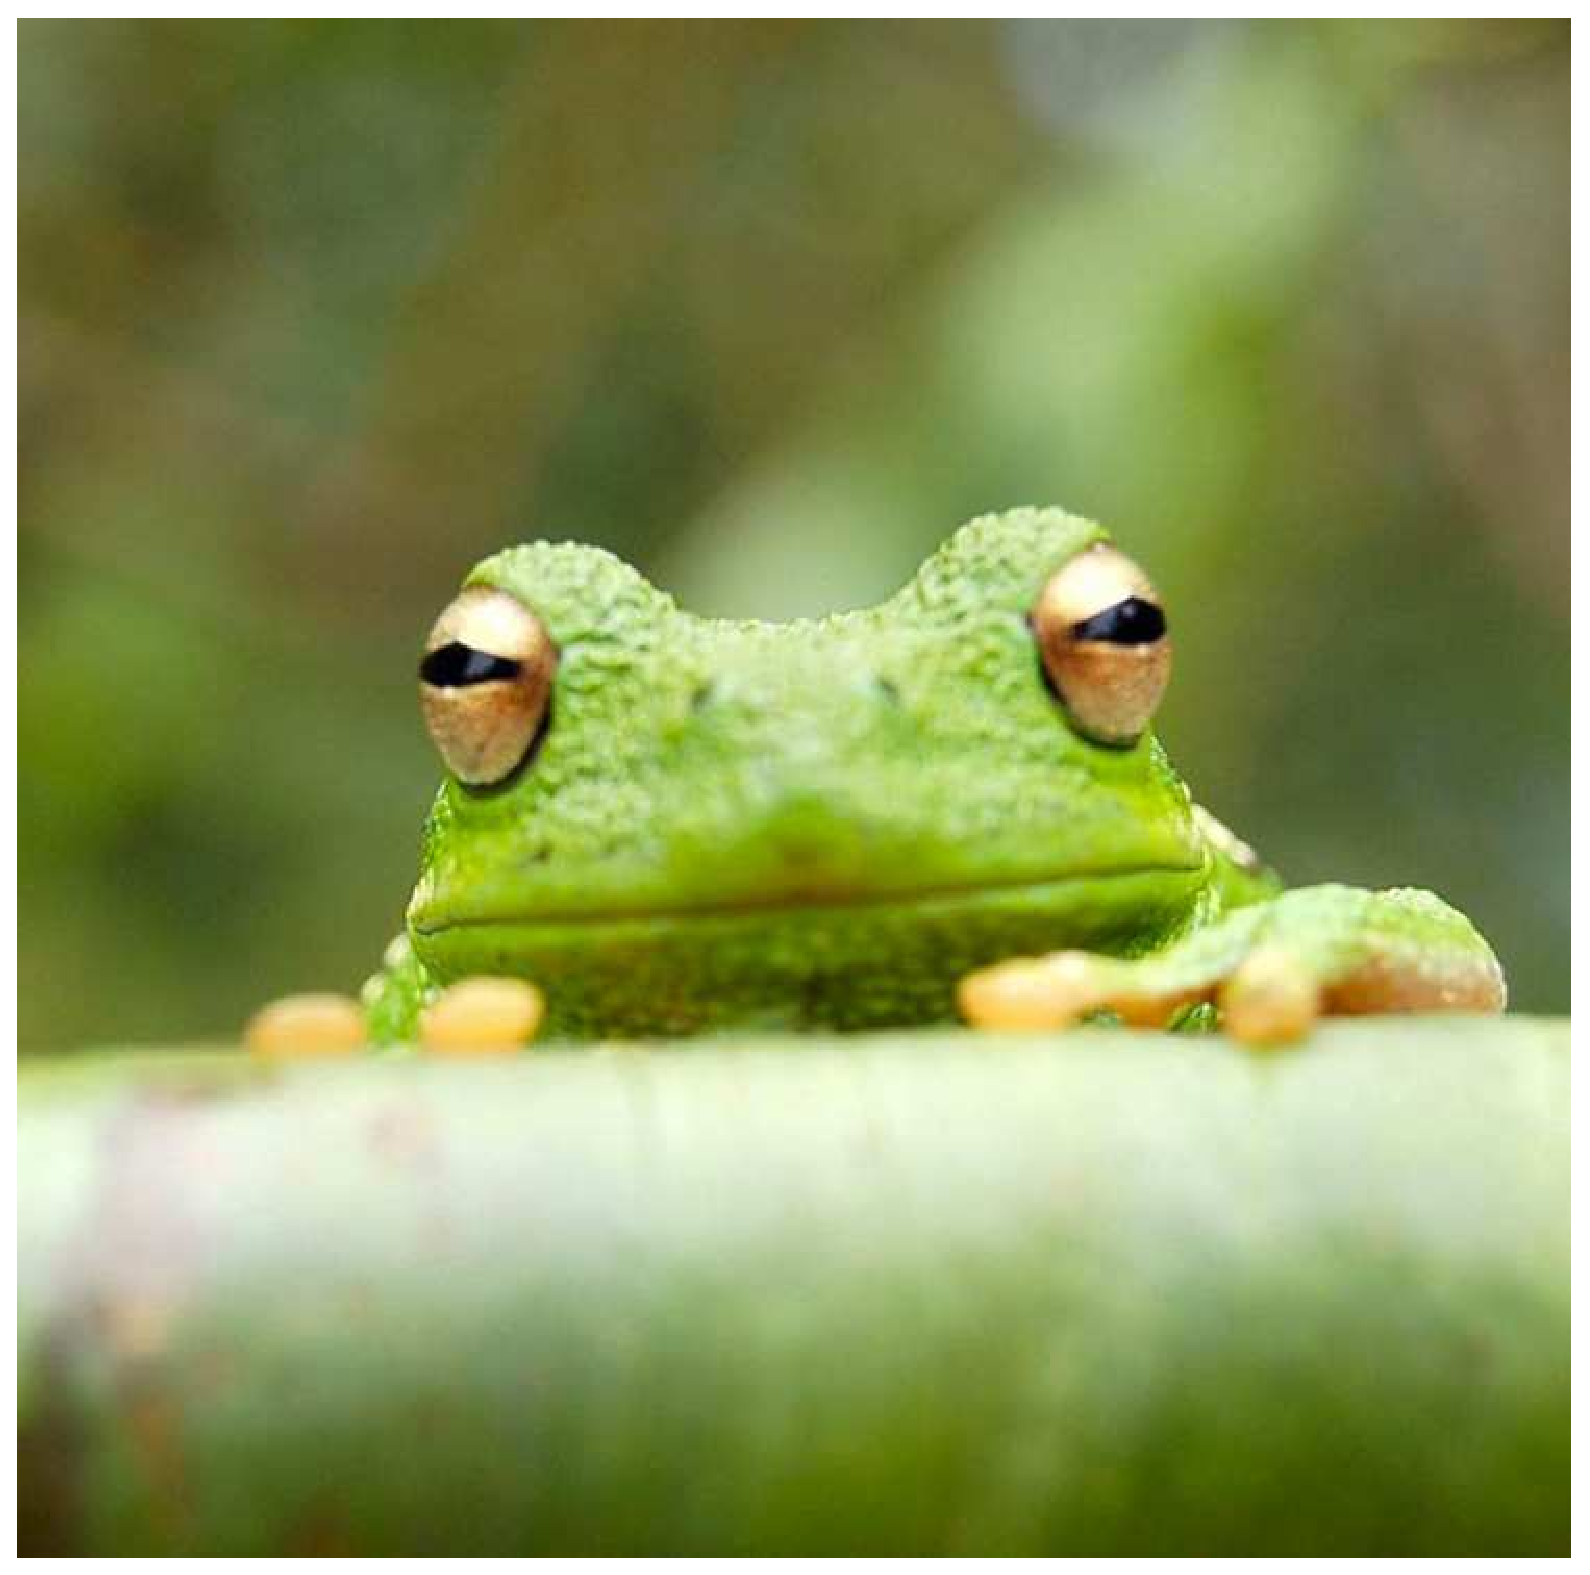
\includegraphics[width=.8\linewidth]{frog}
%\caption{Placeholder image of a frog with a long example caption to show justification setting.}
%\label{fig:frog}
%\end{figure}
%
%\subsection*{Digital Figures}
%\label{sec:figures}
%
%Figure \ref{fig:frog} shows an example of how to insert a column-wide figure. To insert a figure wider than one column, please use the \verb|\begin{figure*}...\end{figure*}| environment. Figures wider than one column should be sized to 11.4 cm or 17.8 cm wide.
%
%%% Do not use widetext if paper is in single column.
%\begin{widetext}
%\begin{align*}
%(x+y)^3&=(x+y)(x+y)^2\\
%       &=(x+y)(x^2+2xy+y^2) \numberthis \label{eqn:example} \\
%       &=x^3+3x^2y+3xy^3+x^3. 
%\end{align*}
%\end{widetext}

%\subsection*{Supporting Information (SI)}
%
%The main text of the paper must stand on its own without the SI. Refer to SI in the manuscript at an appropriate point in the text. Number supporting figures and tables starting with S1, S2, etc. Authors are limited to no more than 10 SI files, not including movie files. Authors who place detailed materials and methods in SI must provide sufficient detail in the main text methods to enable a reader to follow the logic of the procedures and results and also must reference the online methods. If a paper is fundamentally a study of a new method or technique, then the methods must be described completely in the main text. Because PNAS edits SI and composes it into a single PDF, authors must provide the following file formats only.


%\subsubsection*{SI Figures}

\matmethods{We here describe in detail our calculation of bin-averaged flux divergence profiles from GCM output. Note that all data used in constructing all the figures presented here can be found at https://github.com/jeevanje/rad\_cooling. 

For a GCM column at a given longitude, latitude, and time (we use monthly mean output), we must first identify a range of tropospheric model levels $k$ over which the temperature $T$ varies monotonically. We identify the uppermost of these levels \kmax\ as the minimum  $k>10$ for which $T[k+1]>T[k]$. If none such exists (i.e. no stratospheric inversion) then $\kmax$ takes its highest possible value (i.e. model top).
The minimum $k$ value $\kmin$ equals 1 if there is no inversion below \kmax, and otherwise is the largest $k< \kmax$ such that $T[k]>T[k-1]$. We then interpolate the column's SW and LW radiative fluxes over this $T$ range onto a uniform $T$ grid running from 150 to 350 K in increments of 2 K, and assign these interpolated profiles, weighted by column area,  to the appropriate \Ts\ bin using $T[1]$ (where \Ts-binning is done with the same uniform grid as for vertical levels $T$). We repeat this for each GCM column over the last 30 years of each simulation, keeping track of the accumulated column area for each bin and $T$ level. This allows us to produce an area-weighted average flux profile in each bin, where in a given bin the total area represented at each $T$ level drops off at lower and higher $T$  (due to small variations in $T[\kmin]$ and $T[\kmax]$ within the bin). These average flux profiles (one per bin) may then be differentiated with respect to $T$, yielding the $-\ppt \Fnet$ profiles shown in Fig. \ref{fnet_ipsl} and \ref{fnet_all}. To reduce artifacts from binning, the profiles are cut off once the total area at a given $T$ is less than 90\% of the maximum value in the vertical (where this maximum value is taken throughout most of that bin's tropospheric $T$ range, as expected). 
%Also, for consistency with Figs. \ref{pptflw_tinv_dam} and \ref{pptfsw_tinv_dam} where profiles are only plotted above $\Tlcl \approx \Ts - 5$ K , we cut off each GCM profile at \Ts - 5 K.

The decomposition of these net flux divergence profiles into their LW and SW components is given in SI Appendix, Fig. S12, which shows that  \Ts-invariance aloft holds for the LW and SW separately in the GCMs, just as for the CRM. }

\showmatmethods % Display the Materials and Methods section

\acknow{Thanks are due to Tim Merlis, Mark Cane, Jake Seeley,  David Paynter, Yi Ming, and Leo Donner for helpful comments during various stages of this work, to Mark Zelinka, Robert Pincus,  and Tim Cronin for encouragement, and to the extraordinarily patient reviewers and editor of this work for their close reading and thoughtful comments. This work was supported by the U.S. Department of Energy's Atmospheric System Research, an Office of Science, Office of Biological and Environmental Research program; Lawrence Berkeley National Laboratory and its National Energy Research Scientific Computing Center (which provided computing resources) are operated for the DOE by the University of California under Contract DE-AC02-05CH11231.}

\showacknow % Display the acknowledgments section

% \pnasbreak splits and balances the columns before the references.
% If you see unexpected formatting errors, try commenting out this line
% as it can run into problems with floats and footnotes on the final page.
\pnasbreak

% Bibliography
\bibliography{library}


\end{document}